%------------------------------------------------------------------------
% Chapter:  Calculation the PDF
%------------------------------------------------------------------------

\chapter{PDF calculation \label{calc}}
\section{Simple PDF calculation \label{calc_pdf}}

Sometimes rather than refining a PDF one simply wants to calculate
one from a structural model e.g. to explore the effect of a certain
parameter on the calculated PDF. Rather than starting a refinement
with no refinement parameters {\it PDFFIT} offers the simple command
{\tt calc} to compute the desired PDFs. As an example we want to
calculate the PDF of $Ni$ with two different termination values
$Q_{max}$. The corresponding sequence of {\it PDFFIT} commands is
shown below.

\footnotesize
\begin{MacVerbatim}
      1 reset
      2 read stru,ni.stru
      3 alloc n,25.0,0.0,1.5,6.5,251
      4 delt[1]=0.3
      5 #
      6 calc
      7 save pdf,1,cal_25.calc
      8 #
      9 qmax[1]=35.0
     10 calc
     11 save pdf,1,cal_35.calc
\end{MacVerbatim}
\normalsize

\noindent The first two command should be familiar already from
the example in section \ref{quick}. In line 3 we allocate the
required space for the PDF we want to calculate without actually
reading any experimental data. The first three parameters of the
{\tt alloc} command are similar to {\it read data} in the earlier
example, they specify the radiation type and values for $Q_{max}$
and the resolution factor $\sigma_{Q}$. The next two values
specify the desired $r$-range which in our example is $1.5$ to
$6.5$\AA. The last parameter is the number of data points we want
which in our example leads to a grid size of $\Delta r =
(6.5-1.5)/(251-1) = 0.02$\AA. In order to see a larger effect, we
set the dynamic correlation factor $\delta$ to a rather large
value in line 4 which gives us quite a sharp first PDF peak. Now
the PDF can be calculated using the command {\tt calc} (line 6)
and the result is saved to the file '{\it cal\_25.calc}' (line 7).
In order to recalculate the same PDF with a different value of
$Q_{max}$, we simply alter the value using the corresponding
variable {\tt qmax[1]} (line 9). Note that the '1' specifies the
number of the data set. Finally we calculate the PDF again (line
10) and save the result to a different file (line 11).

\begin{figure}[!htb]
   \centering
   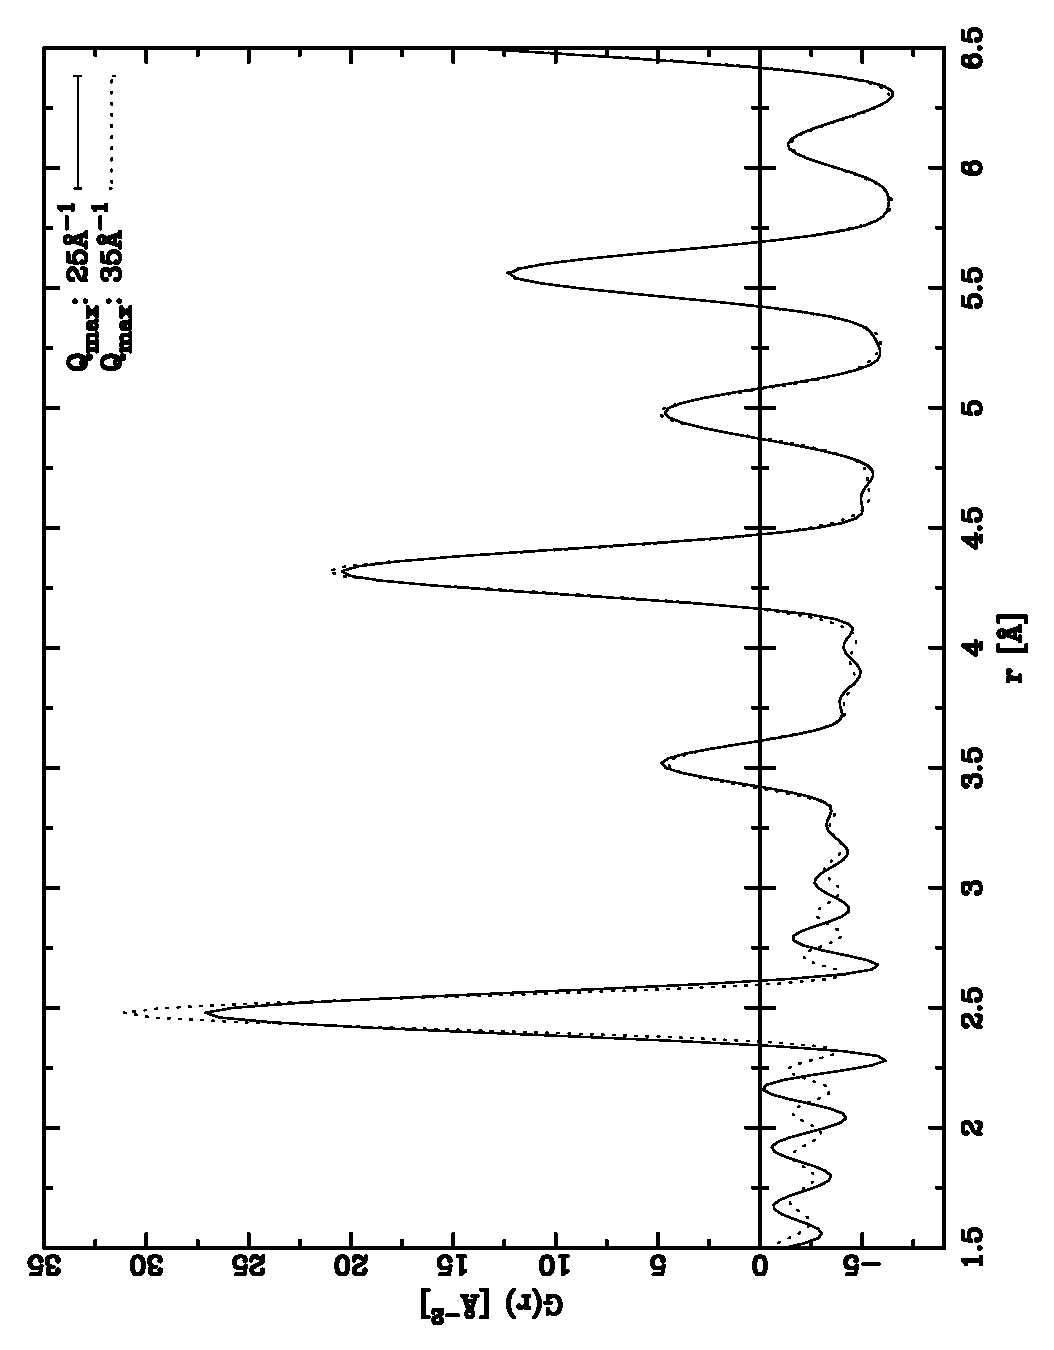
\includegraphics[scale=0.5, angle=270]{cal.1.eps}
   \caption[Calculated PDFs for $Ni$ at different values $Q_{max}$]
           {Calculated PDFs for $Ni$ at different values $Q_{max}$.
            The solid line is the PDF with $Q_{max} = 25$\AA$^{-1}$ and
            the dotted line is for $Q_{max} = 35$\AA$^{-1}$.}
   \label{cal-fig1}
\end{figure}

The result of the example given above is shown in Figure \ref{cal-fig1}.
As one might expect, the termination ripples for the calculation with
the higher $Q_{max}$ show a higher frequency. In addition we can observe
in our particular example that the intrinsic width of the first peak
is smaller than the width of the convolution at $Q_{max}=25$\AA$^{-1}$,
in other words the peak is broadened due to the $Q$ termination.

%------------------------------------------------------------------------
\section{Calculating partial or differential PDFs \label{calc_partial}}

When discussing equation (\ref{eq_igr}) used to calculate the PDF from
a structural model, we just stated that the sum over $ij$ goes over
{\it all} pairs of atoms $i$ and $j$ within the model crystal. This
is perfectly correct to calculate a total PDF. However sometimes it
might be desired to calculate just a partial or differential PDF. Let
us consider $GaAs$ as a simple example. Figure \ref{cal-fig2} shows
the total PDF as well as the differential and partial $Ga$ PDF of
$GaAs$. The total PDF is shown in the top view graph of Figure
\ref{cal-fig2}. Numbering the PDF peaks from the left, we find that
the first peak corresponds to the shortest $Ga-As$ distance. The second
peak is from $Ga-Ga$ and $As-As$ separated by the F-centering, the
next peak is again from $Ga-As$, the fourth peak corresponds to the
lattice repeat and so on. Let us consider just the first two peaks.
A differential PDF contains all pairs of one specific atom, here $Ga$,
and all other atoms. So the first $Ga-As$ peak is the same in the
differential PDF (Fig. \ref{cal-fig2} middle) as in the total one.
The second peak, however, contains contributions of $Ga-Ga$ and
$As-As$ in the total PDF, whereas the differential PDF shows no
$As-As$ pairs. Since there is the same number of both types, the second
peak in the differential PDF has only half the height compared to
the total PDF. The partial $Ga$ PDF (Fig. \ref{cal-fig2} bottom) contains
only contributions of $Ga-Ga$ pairs. Thus the first peak is missing
whereas the second peak is equivalent to the one observed in the
differential PDF. \par

\begin{figure}[!htb]
   \centering
   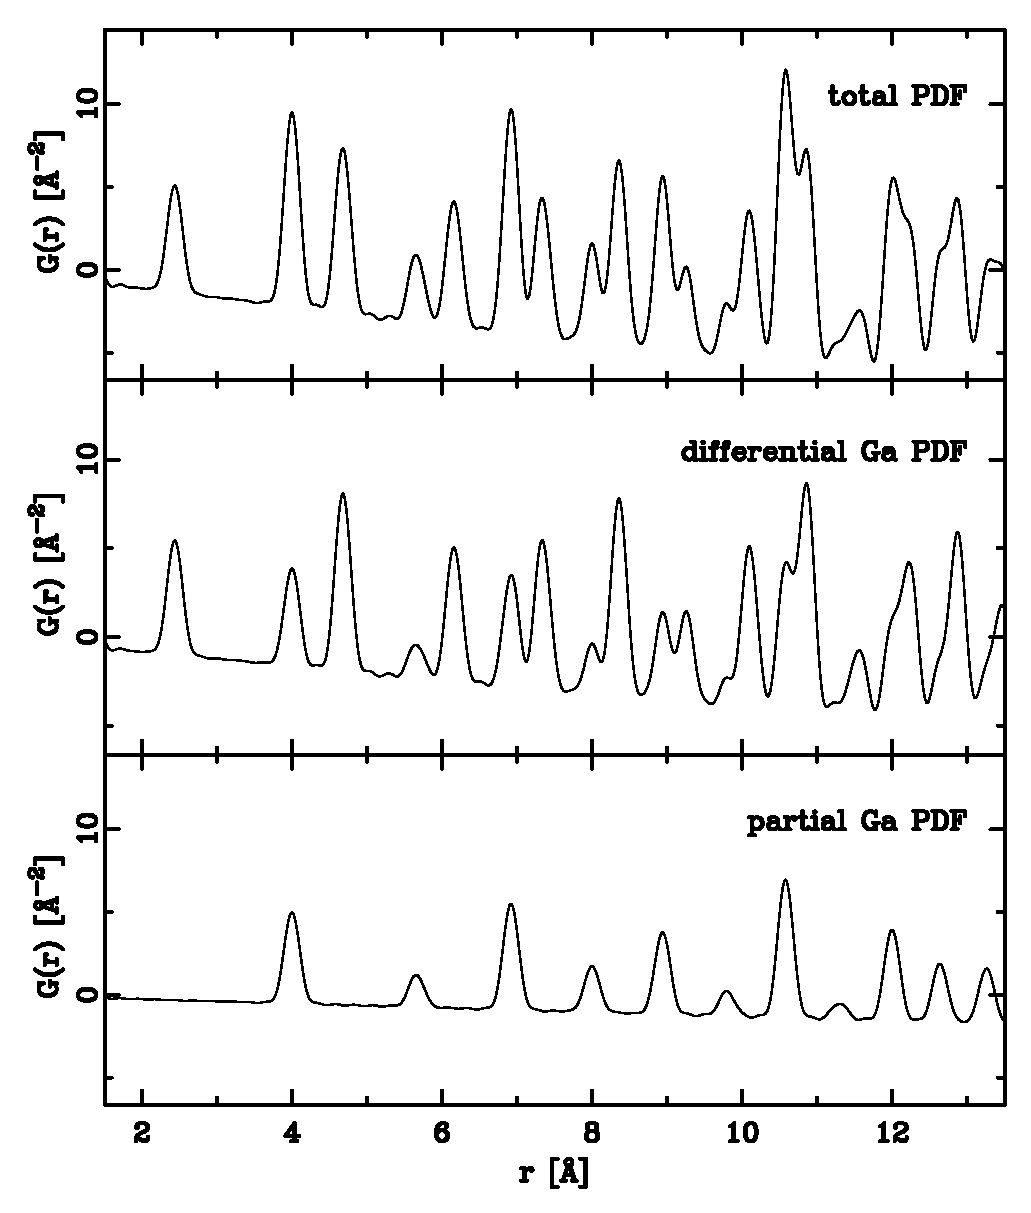
\includegraphics[scale=0.6, angle=0]{cal.2.eps}
   \caption[Total, differential and partial PDF of $GaAs$]
           {Top: Total $GaAs$ PDF. Middle: Differential $Ga$ PDF of
            $GaAs$. Bottom: Partial $Ga$ PDF of $GaAs$.}
   \label{cal-fig2}
\end{figure}

The determination which atoms contribute to which peaks in the PDF
is not always as simple as in our $GaAs$ example and the calculation
of various partial PDFs might help to understand a more complex
PDF. \par

The macro that was used to calculate the PDFs shown in Figure \ref{cal-fig2}
is listed below. Again the line number were added for convenience. The
first three lines are similar to the example in the last section. The
commands to select particular atom types are {\tt isel} and {\tt jsel}.

\footnotesize
\begin{MacVerbatim}
      1 reset
      2 read stru,gaas.stru
      3 alloc x,25.0,0.0,1.5,13.5,601
      4 #
      5 isel 1,all
      6 jsel 1,all
      7 calc
      8 save pdf,1,tot.calc
      9 #
     10 ides 1,all
     11 jdes 1,all
     12 isel 1,ga
     13 jsel 1,all
     14 calc
     15 save pdf,1,dif_ga.calc
     16 #
     17 ides 1,all
     18 jdes 1,all
     19 isel 1,ga
     20 jsel 1,ga
     21 calc
     22 save pdf,1,par_ga.calc
\end{MacVerbatim}
\normalsize

\noindent To calculate the total PDF, we simply select all atom
types present in the structure (lines 5--6) and calculate and save
the PDF (lines 7--8). Note that the selection of all atoms is the
default when starting {\it PDFFIT} or using the command {\tt
reset}. The first parameter of the {\tt i/jsel} and {\tt i/jdes}
commands is the corresponding data set number, here simply one. To
calculate the differential PDF we select $Ga$ for atom $i$ (line
12) and all atoms for atom $j$ (line 13). Since the command {\tt
isel} or {\tt jsel} adds the specified atom to the list of allowed
atoms, we need to deselect all previously selected atoms first as
done in lines 10--11 of our example. Again we calculate and save
the new PDF (lines 14--15). Finally we select just $Ga$ for atoms
$i$ and $j$ (lines 17--20) to obtain the partial $Ga$ PDF and
recalculate and save the result (lines 21-22). \par

Note, that {\it PDFFIT} can also refine a experimental differential PDF
which for example can be obtained from anomalous X-ray scattering. The
required commands to select the specific atom types are exactly the same
as in this example. Note, that {\it PDFFIT} normalizes the number density
$\rho_{0}$ by a weighting factor given below:

\begin{equation}
  w(kl) = \frac{\sum_{kl} c_{k}c_{l}b_{k}b_{l}}
               {\sum_{ij} c_{i}c_{j}b_{i}b_{j}}
  \label{eq_norm}
\end{equation}

Here the sum over $kl$ is only over those atom that are selected
and contribute to the PDF whereas $ij$ sums over all atoms within the
crystal. It is immediately obvious that $w(kl)=1.0$ for the total
PDF. This definition is consistent with the use of Faber-Ziman
partial structure factors. For details refer to \cite{waseda} and
appendix \ref{app-deriv}.

%------------------------------------------------------------------------
